\documentclass[14pt]{extbook}
\usepackage{multicol, enumerate, enumitem, hyperref, color, soul, setspace, parskip, fancyhdr} %General Packages
\usepackage{amssymb, amsthm, amsmath, latexsym, units, mathtools} %Math Packages
\everymath{\displaystyle} %All math in Display Style
% Packages with additional options
\usepackage[headsep=0.5cm,headheight=12pt, left=1 in,right= 1 in,top= 1 in,bottom= 1 in]{geometry}
\usepackage[usenames,dvipsnames]{xcolor}
\usepackage{dashrule}  % Package to use the command below to create lines between items
\newcommand{\litem}[1]{\item#1\hspace*{-1cm}\rule{\textwidth}{0.4pt}}
\pagestyle{fancy}
\lhead{Progress Quiz 6}
\chead{}
\rhead{Version A}
\lfoot{1430-1829}
\cfoot{}
\rfoot{test}
\begin{document}

\begin{enumerate}
\litem{
Solve the radical equation below. Then, choose the interval(s) that the solution(s) belongs to.\[ \sqrt{-6 x^2 - 24} - \sqrt{25 x} = 0 \]\begin{enumerate}[label=\Alph*.]
\item \( \text{All solutions lead to invalid or complex values in the equation.} \)
\item \( x \in [-2.1,-1.01] \)
\item \( x \in [-2.72,-2.4] \)
\item \( x_1 \in [2.51, 2.69] \text{ and } x_2 \in [0.5,4.5] \)
\item \( x_1 \in [-2.72, -2.4] \text{ and } x_2 \in [-2.5,-0.5] \)

\end{enumerate} }
\litem{
What is the domain of the function below?\[ f(x) = \sqrt[4]{-9 x - 4} \]\begin{enumerate}[label=\Alph*.]
\item \( (-\infty, a], \text{where } a \in [-3.39, -1.49] \)
\item \( (-\infty, \infty) \)
\item \( (-\infty, a], \text{ where } a \in [-0.9, 0.29] \)
\item \( [a, \infty), \text{where } a \in [-1.44, 2.56] \)
\item \( [a, \infty), \text{where } a \in [-9.25, -1.25] \)

\end{enumerate} }
\litem{
Solve the radical equation below. Then, choose the interval(s) that the solution(s) belongs to.\[ \sqrt{6 x - 3} - \sqrt{-2 x - 4} = 0 \]\begin{enumerate}[label=\Alph*.]
\item \( x \in [-0.1,1] \)
\item \( x_1 \in [-4.9, -1.6] \text{ and } x_2 \in [-3.5,1.5] \)
\item \( \text{All solutions lead to invalid or complex values in the equation.} \)
\item \( x_1 \in [-0.4, 0.6] \text{ and } x_2 \in [-3.5,1.5] \)
\item \( x \in [-0.4,0.6] \)

\end{enumerate} }
\litem{
Solve the radical equation below. Then, choose the interval(s) that the solution(s) belongs to.\[ \sqrt{-7 x - 7} - \sqrt{-8 x + 6} = 0 \]\begin{enumerate}[label=\Alph*.]
\item \( x \in [11.9,15.8] \)
\item \( \text{All solutions lead to invalid or complex values in the equation.} \)
\item \( x_1 \in [-1.4, 0.8] \text{ and } x_2 \in [9,16] \)
\item \( x_1 \in [-1.4, 0.8] \text{ and } x_2 \in [-3.25,3.75] \)
\item \( x \in [0.8,3.3] \)

\end{enumerate} }
\litem{
Choose the graph of the equation below.\[ f(x) = - \sqrt[3]{x - 10} - 5 \]\begin{enumerate}[label=\Alph*.]
\begin{multicols}{2}\item 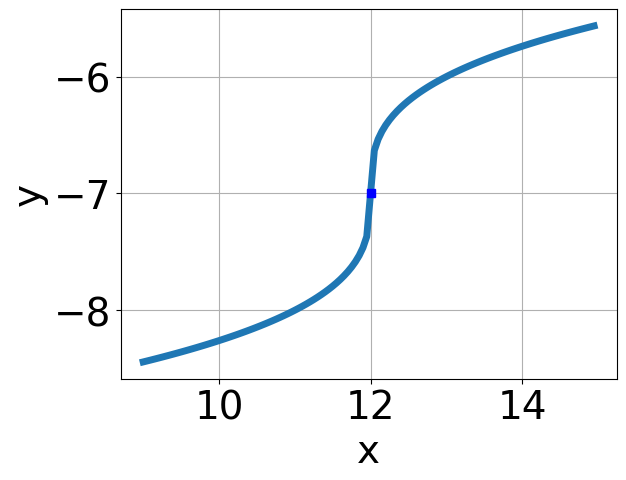
\includegraphics[width = 0.3\textwidth]{../Figures/radicalEquationToGraphAA.png}\item 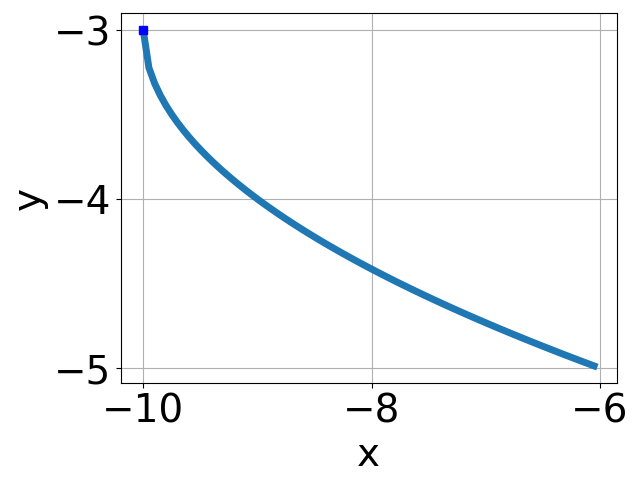
\includegraphics[width = 0.3\textwidth]{../Figures/radicalEquationToGraphBA.png}\item 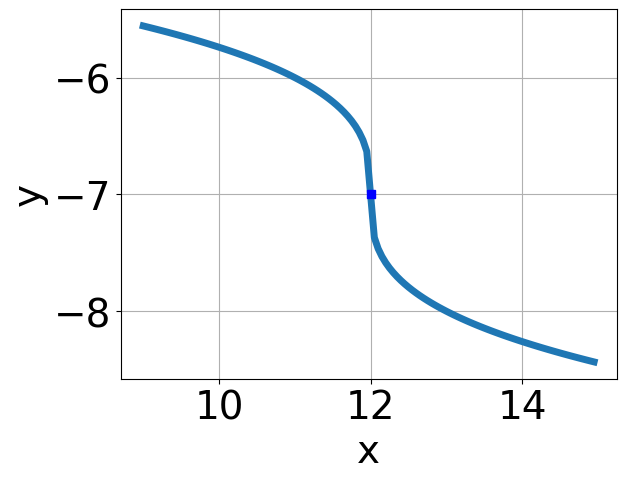
\includegraphics[width = 0.3\textwidth]{../Figures/radicalEquationToGraphCA.png}\item 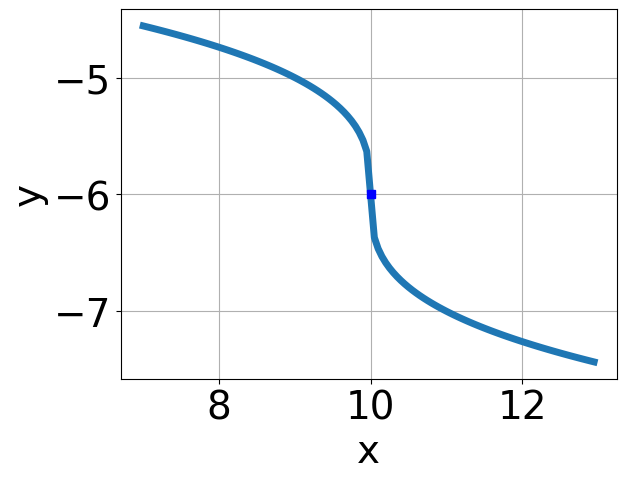
\includegraphics[width = 0.3\textwidth]{../Figures/radicalEquationToGraphDA.png}\end{multicols}\item None of the above.
\end{enumerate} }
\litem{
Choose the equation of the function graphed below.
\begin{center}
    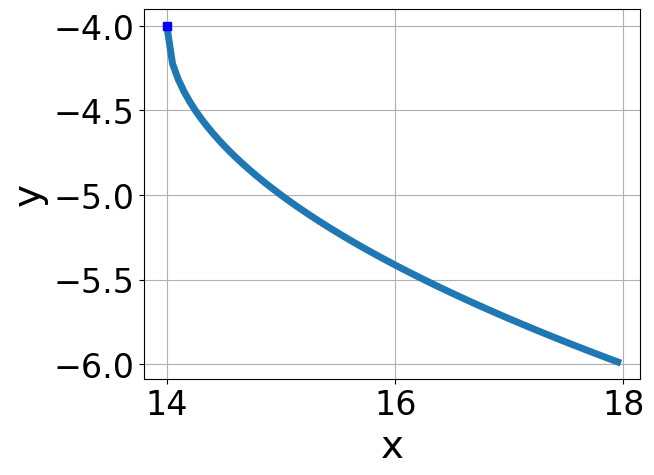
\includegraphics[width=0.5\textwidth]{../Figures/radicalGraphToEquationCopyA.png}
\end{center}
\begin{enumerate}[label=\Alph*.]
\item \( f(x) = - \sqrt[3]{x - 10} + 7 \)
\item \( f(x) = - \sqrt[3]{x + 10} + 7 \)
\item \( f(x) = \sqrt[3]{x - 10} + 7 \)
\item \( f(x) = \sqrt[3]{x + 10} + 7 \)
\item \( \text{None of the above} \)

\end{enumerate} }
\litem{
What is the domain of the function below?\[ f(x) = \sqrt[3]{3 x - 6} \]\begin{enumerate}[label=\Alph*.]
\item \( \text{The domain is } (-\infty, a], \text{   where } a \in [1, 4] \)
\item \( (-\infty, \infty) \)
\item \( \text{The domain is } (-\infty, a], \text{   where } a \in [-2.5, 1.5] \)
\item \( \text{The domain is } [a, \infty), \text{   where } a \in [1, 6] \)
\item \( \text{The domain is } [a, \infty), \text{   where } a \in [0.5, 1.5] \)

\end{enumerate} }
\litem{
Choose the equation of the function graphed below.
\begin{center}
    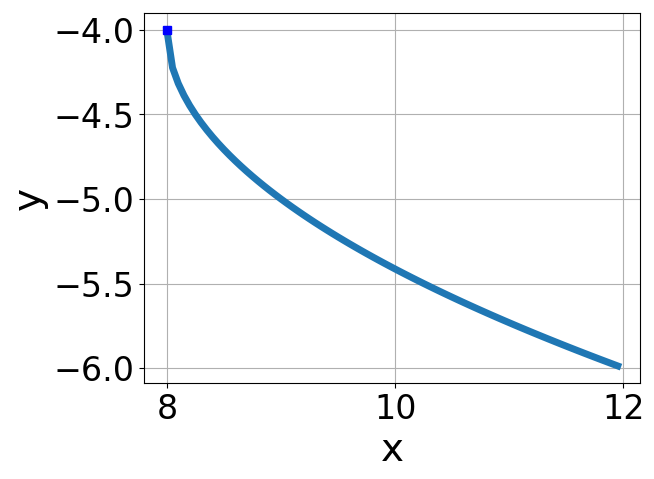
\includegraphics[width=0.5\textwidth]{../Figures/radicalGraphToEquationA.png}
\end{center}
\begin{enumerate}[label=\Alph*.]
\item \( f(x) = - \sqrt[3]{x - 10} - 7 \)
\item \( f(x) = \sqrt[3]{x - 10} - 7 \)
\item \( f(x) = - \sqrt[3]{x + 10} - 7 \)
\item \( f(x) = \sqrt[3]{x + 10} - 7 \)
\item \( \text{None of the above} \)

\end{enumerate} }
\litem{
Solve the radical equation below. Then, choose the interval(s) that the solution(s) belongs to.\[ \sqrt{-40 x^2 - 18} - \sqrt{61 x} = 0 \]\begin{enumerate}[label=\Alph*.]
\item \( x \in [-1.53,-0.98] \)
\item \( x_1 \in [0.81, 1.41] \text{ and } x_2 \in [0.37,0.89] \)
\item \( x_1 \in [-1.53, -0.98] \text{ and } x_2 \in [-0.49,0.22] \)
\item \( \text{All solutions lead to invalid or complex values in the equation.} \)
\item \( x \in [-0.76,-0.32] \)

\end{enumerate} }
\litem{
Choose the graph of the equation below.\[ f(x) = - \sqrt{x + 6} - 3 \]\begin{enumerate}[label=\Alph*.]
\begin{multicols}{2}\item 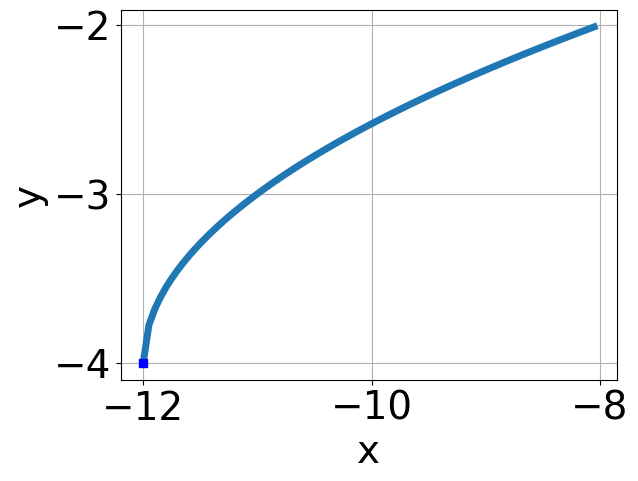
\includegraphics[width = 0.3\textwidth]{../Figures/radicalEquationToGraphCopyAA.png}\item 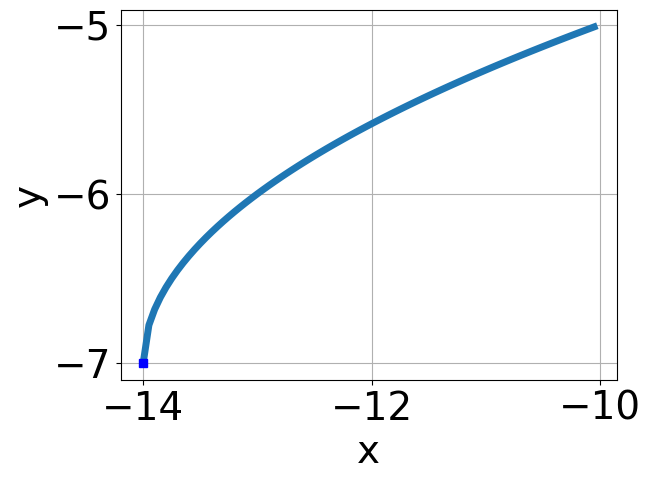
\includegraphics[width = 0.3\textwidth]{../Figures/radicalEquationToGraphCopyBA.png}\item 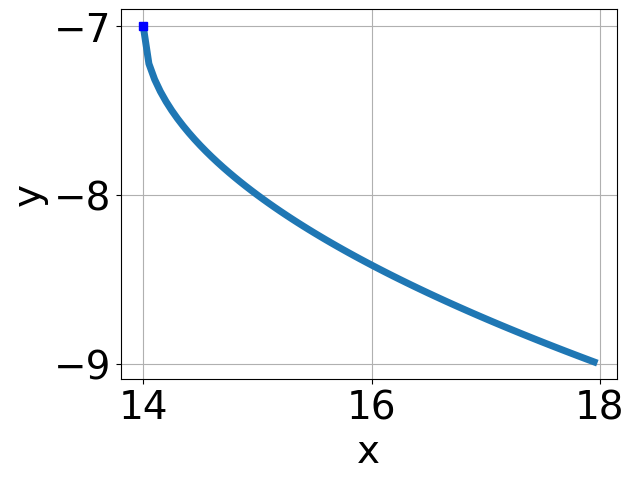
\includegraphics[width = 0.3\textwidth]{../Figures/radicalEquationToGraphCopyCA.png}\item 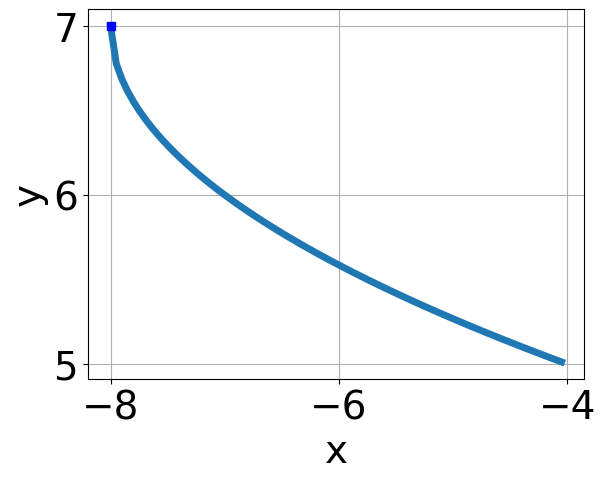
\includegraphics[width = 0.3\textwidth]{../Figures/radicalEquationToGraphCopyDA.png}\end{multicols}\item None of the above.
\end{enumerate} }
\end{enumerate}

\end{document}